\chapter{Aljabar Linier}

\section{Skalar, vektor, matriks, dan tensor}
\subsection{Definisi skalar, vektor, dan matriks}
Berikut ini merupakan definisi praktis dari sudut pandang keilmuan kecerdasan buatan untuk ketiga objek utama di dalam keilmuan aljabar linier ini:
\begin{itemize}
    \item Skalar ($x$): nilai tunggal tanpa dimensi. Formulasi umumnya adalah:
    \begin{equation}\label{eqn:eqn1}
        X
    \end{equation}
    
    Contoh:
    \begin{equation*}
        x = 12
    \end{equation*}
    \item Vektor ($\mathbf{x}$): himpunan bilangan (\textit{array}) berdimensi tunggal yang dapat berupa kolom ataupun baris dan dapat diidentifikasi melalui baris dan kolom.  Formulasi umumnya adalah: 
    \begin{equation}\label{eqn:eqn2}
        \begin{bmatrix}X_{0} & X_{1} & \cdots &  X_{n}\end{bmatrix} \text{ atau } \begin{bmatrix}X_{0} \\ X_{1} \\ \vdots \\ X_{n}\end{bmatrix}
    \end{equation}
    
    Contoh:
    \begin{equation*}
        \mathbf{x} = \begin{bmatrix}1 & 2 & 3\end{bmatrix} \text{ atau } \mathbf{x} = \begin{bmatrix}1 \\ 2 \\ 3\end{bmatrix}
    \end{equation*}
    \item Matriks ($\mathbf{X}$): \textit{Array} berdimensi dua\footnote{Dimensi umumnya didefinisikan dalam format baris, kolom. Matriks merupakan \textit{array} berdimensi dua karena mempunyai baris dan kolom, sementara vektor berdimensi tunggal karena hanya mempunyai baris atau kolom.}, di mana setiap elemennya dapat diakses melalui indeks baris dan kolom\footnote{Pengindeksan yang penyusun gunakan pada catatan ini berbeda dengan kebanyakan pengindeksan yang dijabarkan pada buku teks aljabar linier karena dalam kontek kecerdasan buatan yang lebih dekat pada dunia ilmu komputer, umumnya digunakan pengindeksan yang dimulai dari nol.}. Formulasi umumnya adalah:
    \begin{equation}\label{eqn:eqn3}
        \textbf{X} = \begin{bmatrix}X_{0,0} & X_{0,1} & \cdots & X_{0,n}\\X_{1,0} & X_{1,1} & \cdots & X_{1,n}\\ \cdots & \cdots & \cdots & \cdots \\X_{m,0} & X_{m,1} & \cdots & X_{m,n} \end{bmatrix}
    \end{equation}
    
    Contoh:
    \begin{equation*}
        \textbf{X} = \begin{bmatrix}1 & 2 & 3\\4 & 5 & 6\end{bmatrix}
    \end{equation*}
\end{itemize}

\subsection{Operasi antar matriks}
Operasi matriks seperti penjumlahan, pengurangan, dan perkalian sangat lazim dijumpai di dalam algoritma pemelajaran mesin.
\subsubsection{Penjumlahan dan Pengurangan Matriks}
Penjumlahan atau pengurangan matriks merupakan operasi penjumlahan atau pengurangan antar elemen dengan indeks yang sama pada kedua matriks, oleh karena itu prasyarat utamanya adalah kedua matriks yang hendak dijumlahkan harus mempunyai dimensi yang sama. Penjumlahan atau pengurangan antar matriks $\mathbf{A}$ dan $\mathbf{B}$ akan menghasilkan matriks $\mathbf{C}$ dengan dimensi yang sama. Berikut adalah formulasi umum operasi penjumlahan atau pengurangan antar matriks tersebut:
\begin{dmath}\label{eqn:eqn4}
    \textbf{A} \pm \textbf{B} = \begin{bmatrix}a_{0,0} & a_{0,1} & \cdots & a_{0,n}\\ a_{1,0} & a_{1,1} & \cdots & a_{1,n} \\ \vdots & \vdots & \ddots & \vdots \\ a_{m,0} & a_{m,1} & \cdots & a_{m,n}\end{bmatrix} + \begin{bmatrix}b_{0,0} & b_{0,1} & \cdots & b_{0,n}\\ b_{1,0} & b_{1,1} & \cdots & b_{1,n} \\ \vdots & \vdots & \ddots & \vdots \\ b_{m,0} & b_{m,1} & \cdots & b_{m,n}\end{bmatrix} = \begin{bmatrix}a_{0,0} \pm b_{0,0} & a_{0,1} \pm b_{0,1} & \cdots & a_{0,n} \pm b_{0,n}\\ a_{1,0} \pm b_{1,0} & a_{1,1} \pm b_{1,1} & \cdots & a_{1,n} \pm b_{1,n} \\ \vdots & \vdots & \ddots & \vdots \\ a_{m,0} \pm b_{m,0} & a_{m,1} \pm b_{m,1} & \cdots & a_{m,n} \pm b_{m,n}\end{bmatrix}
\end{dmath}

Contoh:
\begin{equation*}
    \textbf{A} + \textbf{B} = \begin{bmatrix}1 & 2 & 3 \\ 4 & 5 & 6\end{bmatrix} + \begin{bmatrix}2 & 1 & 4\\ 1 & 1 & 2\end{bmatrix} = \begin{bmatrix}3 & 3 & 7 \\ 5 & 6 & 8 \end{bmatrix}
\end{equation*}

\begin{equation*}
    \mathbf{A} - \mathbf{B} = \begin{bmatrix}1 & 2 & 3 \\ 4 & 5 & 6\end{bmatrix} - \begin{bmatrix}2 & 1 & 4\\ 1 & 1 & 2\end{bmatrix} = \begin{bmatrix}-1 & 1 & -1 \\ 3 & 4 & 4\end{bmatrix}
\end{equation*}

\subsubsection{Perkalian matriks}
Perkalian antar matriks $\mathbf{A}$ dan $\mathbf{B}$ akan menghasilkan matriks baru, yakni $\mathbf{C}$. Untuk melakukan operasi perkalian ini, matriks $\mathbf{A}$ harus mempunyai jumlah kolom yang sama dengan jumlah baris pada matriks $\mathbf{B}$. Berikut adalah formulasi umum perkalian antar kedua matriks:

\begin{dmath*}
    \begin{bmatrix}a_{0,0} & a_{0,1}\\ a_{1,0} & a_{1,1}\end{bmatrix} * \begin{bmatrix} b_{0,0} & b_{0,1}\\ b_{1,0} & b_{1,1}\end{bmatrix} =
    \begin{bmatrix}a_{0,0}b_{0,0} + a_{0,1}b_{1,0} & a_{0,0}b_{0,1} + a_{0,1}b_{1,1}\\a_{0,1}b_{0,0} + a_{1,1}b_{1,0} & a_{1,0}b_{0,1} + a_{1,1}b_{1,1} \end{bmatrix} =
    \begin{bmatrix} 
    c_{0,0} & c_{0,1}\\
    c_{1,0} & c_{1,1}
    \end{bmatrix}
\end{dmath*}
Atau secara umum dapat diformulasikan seperti pada persamaan \ref{eqn:eqn5} berikut ini:
\begin{dmath}\label{eqn:eqn5}
    \mathbf{C}_{i,j} = \Sigma_{k} \mathbf{A}_{i,k}\mathbf{B}_{j,k}
\end{dmath}
Perkalian matriks juga dapat terjadi pada matriks yang mempunyai dimensi yang berbeda, asalkan matriks pertama mempunyai kolom yang sama dengan jumlah baris pada matriks kedua,seperti pada contoh berikut ini:
\begin{dmath*}
    \begin{bmatrix}1 & 2\\3 & 4\\5 & 6\end{bmatrix} * \begin{bmatrix}1 & 3 & 5\\2 & 4 & 6\end{bmatrix} = \begin{bmatrix}1(1) + 2(2) & 1(3) + 2(4) & 1(5) + 2(6)\\3(1) + 4(2) & 3(3) + 4(4) & 3(5) + 4(6)\\ 5(1) + 6(2) & 5(3) + 6(4) & 5(5) + 6(6)\end{bmatrix} = \begin{bmatrix}5 & 11 & 17\\11 & 25 & 39\\17 & 39 & 61\end{bmatrix}
\end{dmath*}
Terdapat dua buah karakteristik utama dari perkalian matriks, yakni:
\begin{enumerate}
    \item Distributif: 
        \begin{equation} \label{eqn:eqn6}
            \mathbf{A}\left(\mathbf{B} + \mathbf{C}\right) = \mathbf{A}\mathbf{B} + \mathbf{A}\mathbf{C}
        \end{equation}
    \item Asosiatif: 
        \begin{equation}\label{eqn:eqn7}
            \mathbf{A}\left(\mathbf{B}\mathbf{C}\right) = \left(\mathbf{A}\mathbf{B}\right)\mathbf{C}
        \end{equation}
\end{enumerate}
\subsection{Transpos}
Transpos merupakan operasi menukar indeks matriks pada diagonal utamanya. Dengan kata lain, transpos menukar indeks baris menjadi indeks kolom, dan sebaliknya.

Berikut ini adalah contohnya:
\[
    \begin{bmatrix}a_{0,0} & a_{0,1} & a_{0,2}\\ a_{1,0} & a_{1,1} & a_{1,2}\\a_{2,0} & a_{2,1} & a_{2,2}\end{bmatrix}^{T} = \begin{bmatrix}a_{0,0} & a_{1,0} & a_{2,0} \\ a_{0,1} & a_{1,1} & a_{2,1} \\ a_{0,2} & a_{1,2} & a_{2,2}\end{bmatrix}
\]

\[
\begin{bmatrix}1 & 2 & 3\\4 & 5 & 6\\7 & 8 & 9\end{bmatrix} = \begin{bmatrix} 1 & 4 & 7 \\ 2 & 5 & 8\\ 3 & 6 & 9\end{bmatrix}
\]

Berikut ini merupakan contoh operasi transpos pada matriks dengan dimensi baris dan kolom yang berbeda:

\[
\begin{bmatrix}1 & 2 \\ 3 & 4 \\ 5 & 6\end{bmatrix}^{T} = \begin{bmatrix}1 & 3 & 5\\2 & 4 & 6\end{bmatrix}
\]

Kita juga dapat melakukan operasi transpos pada vektor. Operasi transpos vektor ini lah yang sering digunakan dalam pemrosesan dan pembersihan data sebelum dijadikan input algoritma pemelajaran mesin:

\[
\begin{bmatrix} 1 & 2 & 3\end{bmatrix}^{T} = \begin{bmatrix} 1\\2\\3\end{bmatrix}
\]


\subsection{Tensor}
Terkadang di dalam era data raksasa seperti saat ini, kita harus berurusan dengan data yang mempunyai sumbu dimensi lebih dari dua. Data dengan sumbu dimensi banyak inilah yang dinamakan tensor (vektor dan matriks juga termasuk ke dalam tensor dimensi satu dan dua, lihat Gambar \ref{fig:fig1}) . Operasi dan fitur yang ditawarkan oleh tensor sama seperti yang telah kita ketahui pada vektor dan matriks, hanya saja berbeda pada dimensi saja, dan hal ini dapat dengan mudah diatasi oleh kemajuan fasilitas komputasi numerik saat ini.

\begin{figure}[H]
    \centering
    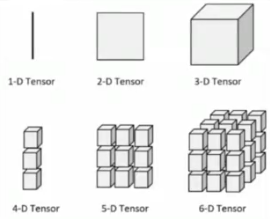
\includegraphics[width=0.5\textwidth]{gambar/gmb1.png}
    \caption{Ilustrasi tensor.}
    \label{fig:fig1}
\end{figure}

\section{Laboratorium 1: skalar, vektor, matriks, dan tensor}
Pada bagian ini, kita akan mencoba untuk mengimplementasikan konsep - konsep yang telah kita pelajari di lingkungan komputasi Python, khususnya dengan menggunakan pustaka numerik NumPy. Untuk itu, kita harus memastikan bahwa lingkungan yang kita gunakan telah sesuai, jalankan perintah berikut ini di Jupyter Notebook kalian masing - masing:

\subsection{Memulai sesi NumPy}
\begin{pyin}
import sys
import numpy as np

print("Python: {}".format(sys.version))
print("NumPy: {}".format(np.__version__))
\end{pyin}

\begin{pyin}
Python: 3.8.3 (default, May 19 2020, 18:47:26) 
[GCC 7.3.0]
NumPy: 1.18.1
\end{pyin}

Kita dapat mendefinisikan skalar (yang mana merupakan nilai bilangan tunggal) dengan menggunakan operator \verb|=| untuk penugasan ke suatu variabel tertentu:

\begin{pyin}
# penugasan skalar
x = 128
x
\end{pyin}

\begin{pyout}
128
\end{pyout}

Dengan NumPy, kita dapat mendefinisikan vektor dengan menggunakan fungsi \verb|array()|:
\begin{pyin}
# penugasan vektor
x = np.array((1,2,8))
x
\end{pyin}
\begin{pyout}
array([1, 2, 8])
\end{pyout}

\textit{Array} mempunyai beberapa atribut yang dapat memberitahu kita tentang informasi terkait dimensi dan ukuran suatu vektor:

\begin{pyin}
print("Dimensi vektor: {}".format(x.shape))
print("Ukuran vektor: {}".format(x.size))
\end{pyin}
\begin{pyout}
Dimensi vektor: (3,)
Ukuran vektor: 3
\end{pyout}

Untuk mendefinisikan matriks, kita dapat menggunakan fungsi \verb|matrix()| di pustaka NumPy. Guna memisahkan baris antar matriksnya, kita dapat menggunakan tanda \verb|[]| dan koma:

\begin{pyin}
X = np.matrix([[1,2,8],[2,2,0],[3,2,0]])
X
\end{pyin}
\begin{pyout}
matrix([[1, 2, 8],
        [2, 2, 0],
        [3, 2, 0]])        
\end{pyout}


Untuk mengetahui dimensi dan ukuran matriks $X$, kita dapat menggunakan perintah yang sama:

\begin{pyin}
print('Dimensi matriks: {}'.format(X.shape))
print('Ukuran matriks: {}'.format(X.size))
\end{pyin}
\begin{pyout}
Dimensi matriks: (3, 3)
Ukuran matriks: 9
\end{pyout}
NumPy memudahkan kita untuk mendefinisikan matriks secara cepat, misalkan pada kasus ini kita hendak mendefinisikan matriks identitas $3 \times 3$, kita tinggal menggunakan fungsi \verb|ones()|:
\begin{pyin}
X = np.ones((3,3))
X
\end{pyin}
\begin{pyout}
array([[1., 1., 1.],
       [1., 1., 1.],
       [1., 1., 1.]])
\end{pyout}

\begin{pyin}
print('Dimensi matriks: {}'.format(X.shape))
print('Ukuran matriks: {}'.format(X.size))
\end{pyin}

\begin{pyout}
Dimensi matriks: (3, 3)
Ukuran matriks: 9
\end{pyout}

Sebagai manusia yang hidup di ruang tiga dimensi, tentu kita akan sangat kesulitan ketika memvisualisasikan tensor berdimensi banyak, namun NumPy mempermudah kita untuk melakukan pendefinisian ini dengan menggunakan satu baris perintah:
\begin{pyin}
X = np.ones((3,3,3))
X
\end{pyin}
\begin{pyout}
array([[[1., 1., 1.],
        [1., 1., 1.],
        [1., 1., 1.]],

       [[1., 1., 1.],
        [1., 1., 1.],
        [1., 1., 1.]],

       [[1., 1., 1.],
        [1., 1., 1.],
        [1., 1., 1.]]])
\end{pyout}
\begin{pyin}
print("Dimensi tensor: {}".format(x.shape))
print("Ukuran tensor: {}".format(x.size))
\end{pyin}
\begin{pyout}
Dimensi tensor: (3,)
Ukuran tensor: 3
\end{pyout}
\subsection{Pengindeksan}
Bagian ini mencoba untuk memfamiliarkan konvensi pengindeksan NumPy.
\begin{pyin}
A = np.ones((5,5), dtype = np.int)
print(A)
\end{pyin}

\begin{pyout}
\%[[1 1 1 1 1]
 [1 1 1 1 1]
 [1 1 1 1 1]
 [1 1 1 1 1]
 [1 1 1 1 1]]
\end{pyout}
\begin{pyin}
# pengindeksan dimulai dari 0
A[0,1] = 2
print(A)
\end{pyin}
\begin{pyout}
\%[[1 2 1 1 1]
 [1 1 1 1 1]
 [1 1 1 1 1]
 [1 1 1 1 1]
 [1 1 1 1 1]]
\end{pyout}
\begin{pyin}
# Penting untuk dicatat jika NumPy melakukan pengindeksan dengan konvensi baris, kolom 
# Kita dapat melakukan penugasan seluruh baris atau kolom dengan menggunakan operator : 
A[:,0] = 3
print(A)
\end{pyin}
\begin{pyout}
\%[[3 2 1 1 1]
 [3 1 1 1 1]
 [3 1 1 1 1]
 [3 1 1 1 1]
 [3 1 1 1 1]]
\end{pyout}
\begin{pyin}
# Hal ini berlaku juga untuk Tensor berdimensi banyak 
A = np.ones((5,5,5), dtype = np.int)

# Berikut ini contohnya
A[:,0,0] = 128
print(A)
\end{pyin}
\begin{pyout}
\%[[[128   1   1   1   1]
  [  1   1   1   1   1]
  [  1   1   1   1   1]
  [  1   1   1   1   1]
  [  1   1   1   1   1]]

 [[128   1   1   1   1]
  [  1   1   1   1   1]
  [  1   1   1   1   1]
  [  1   1   1   1   1]
  [  1   1   1   1   1]]

 [[128   1   1   1   1]
  [  1   1   1   1   1]
  [  1   1   1   1   1]
  [  1   1   1   1   1]
  [  1   1   1   1   1]]

 [[128   1   1   1   1]
  [  1   1   1   1   1]
  [  1   1   1   1   1]
  [  1   1   1   1   1]
  [  1   1   1   1   1]]

 [[128   1   1   1   1]
  [  1   1   1   1   1]
  [  1   1   1   1   1]
  [  1   1   1   1   1]
  [  1   1   1   1   1]]]
\end{pyout}
\subsection{Operasi antar matriks}
Bagian ini merupakan demo operasi penjumlahan, pengurangan, dan perkalian matriks.
\begin{pyin}
A = np.matrix([[1,2],[3,4]])
B = np.ones((2,2), dtype = np.int)
\end{pyin}
\begin{pyin}
print(A)
\end{pyin}
\begin{pyout}
\%[[1 2]
 [3 4]]
\end{pyout}
\begin{pyin}
print(B)
\end{pyin}
\begin{pyout}
\%[[1 1]
 [1 1]]
\end{pyout}
\begin{pyin}
# Penjumlahan antar elemen
C = A + B
print(C)
\end{pyin}
\begin{pyout}
\%[[2 3]
 [4 5]]
\end{pyout}
\begin{pyin}
# Pengurangan antar elemen
C = A - B
print(C)
\end{pyin}
\begin{pyout}
\%[[0 1]
 [2 3]]
\end{pyout}
\begin{pyin}
# Perkalian matriks
C = A*B
print(C)
\end{pyin}
\begin{pyout}
\%[[3 3]
 [7 7]]
\end{pyout}
\subsection{Transpos matriks}
Seperti yang telah kita pelajari, transpos digunakan untuk menukar elemen antar baris dan kolom pada suatu array. NumPy memudahkan kita untuk melakukan operasi transpos matriks secara efisien.
\begin{pyin}
A = np.array(range(9))
A = A.reshape(3,3)
print(A)
\end{pyin}
\begin{pyout}
\%[[0 1 2]
 [3 4 5]
 [6 7 8]]
\end{pyout}
\begin{pyin}
# operasi transpos
B = A.T
print(B)
\end{pyin}
\begin{pyout}
\%[[0 3 6]
 [1 4 7]
 [2 5 8]]
\end{pyout}
\begin{pyin}
# dengan melakukan double-transpose, maka kita akan mendapatkan matriks awal
C = B.T
print(C)
\end{pyin}
\begin{pyout}
\%[[0 1 2]
 [3 4 5]
 [6 7 8]]
\end{pyout}
\subsection{Tensor berdimensi banyak}
Seperti yang telah dijabarkan sebelumnya, NumPy mempermudah kita untuk melakukan pengolahan data pada tensor berdimensi raksasa. Berikut ini salah satu contoh pendefinisian array berdimensi 10:
\begin{pyin}
A = np.ones((3,3,3,3,3,3,3,3,3,3))
\end{pyin}
\begin{pyin}
print(A.shape)
print(len(A.shape))
print(A.size)
\end{pyin}
\begin{pyout}
(3, 3, 3, 3, 3, 3, 3, 3, 3, 3)
10
59049
\end{pyout}
\section{Norma vektor dan matriks}
Besaran suatu vektor dan matriks dapat diukur menggunakan fungsi yang dikenal sebagai norma (\textit{norm}). Fungsi norma digunakan untuk memetakan suatu vektor ke nilai non-negatif yang menyatakan besaran dari vektor tersebut. Norma vektor $\mathbf{x}$ mengukur jarak antara titik pangkal vektor ke titik $x$. Di dalam dunia kecerdasan buatan norma ini banyak digunakan untuk menghitung fungsi kerugian (\textit{loss function}) pada algoritma jaringan saraf tiruan (\textit{neural networks}). Selain itu, algoritma pemelajaran mesin seperti jaringan pendukung vektor (\textit{Support Vector Machine}: SVM) juga menggunakan norma $L^2$ untuk mengukur jarak antara diskriminan dengan masing - masing vektor pendukung (\textit{support vector}). Formulasi umum dari norma $L^P$ ditunjukkan pada persamaan \ref{eqn:eqn8} berikut ini:
\begin{equation}\label{eqn:eqn8}
 \norm{\mathbf{x}} = \left(\sum_{i}|x_{i}|^{P} \right)^{\frac{1}{P}}   
\end{equation}

Berikut ini adalah beberapa jenis norma yang umum digunakan di dalam penyelesaian algoritma kecerdasan buatan dan pemelajaran mesin:
\subsection{Norma Euklidesan ($L^2$)}
Ketika nilai $P = 2$, maka kita mendapatkan nilai norma Euklidesan atau dikenal juga sebagai norma $L^2$. Formulasi umumnya ditunjukkan pada persamaan \ref{eqn:eqn9} berikut ini:
\begin{equation}\label{eqn:eqn9}
    \norm{\mathbf{x}}_{2} = \left(\sum_{i}|x_{i}|^{2} \right)^{\frac{1}{2}}
\end{equation}
Karena begitu umum untuk digunakan, terkadang kita hanya cukup menuliskannya sebagai $\norm{\mathbf{x}}$. Berikut adalah contoh penggunaan penggunaan norma Euklidesan:
\begin{dmath*}
    \mathbf{x} = [3, 4]\
\end{dmath*}
\begin{dmath*}
    \norm{\mathbf{x}}_{2} = \sqrt{(3)^{2} + (4)^{2}} = 5
\end{dmath*}
Nilai lima merupakan jarak vektor $\mathbf{x}$ dari koordinat awalnya.
\subsection{Norma $L^1$}
Norma ini digunakan pada kasus pembedaan antara nilai non-nol dan nilai nol pada jarak yang sangat kecil diperlukan. Di dalam penerapan algoritma jaringan saraf tiruan di mana dilakukan pembobotan dengan nilai - nilai yang sangat kecil, maka terkadang norma ini diperlukan. Formulasi umumnya ditunjukan pada persamaan \ref{eqn:eqn10} berikut ini:
\begin{equation}\label{eqn:eqn10}
     \norm{\mathbf{x}}_{1} = \sum_{i}|x_{i}|
\end{equation}
\subsection{Norma maksimum ($L^{\infty}$)}
Norma $L^\infty$ atau yang seringkali dikenal sebagai norma maksimum (\textit{max norm}) merupakan norma yang paling banyak dijumpai di dalam kajian kecerdasan buatan dan pemelajaran mesin. Formulasi umumnya ditunjukkan pada persamaan \ref{eqn:eqn11} berikut ini:
\begin{equation}\label{eqn:eqn11}
    \norm{\mathbf{x}}_{\infty} = \max_{i} |x_{i}|
\end{equation}
Meskipun tampak membingungkan, pada dasarnya persamaan \ref{eqn:eqn11} hanya bermakna untuk mencari nilai absolut terbesar dari elemen - elemen vektor $\mathbf{x}$.

\subsection{Norma Frobenius}
Besaran suatu matriks dapat diukur dengan menggunakan norma Frobenius, yang pada dasarnya merupakan norma $L^2$ untuk matriks. Norma Frobenius umum digunakan untuk menganalisis data raksasa seperti pada cabang keilmuan kecerdasan buatan, namun jarang digunakan di luar cabang keilmuan ini. Formulasi umumnya ditunjukkan pada persamaan \ref{eqn:eqn12} berikut ini:
\begin{equation}\label{eqn:eqn12}
    \norm{\mathbf{A}}_{F} = \sqrt{\sum_{i,j}A_{i,j}^{2}}
\end{equation}

\section{Vektor dan matriks spesial}
Pada algoritma kecerdasan buatan dan pemelajaran mesin, kita akan dengan mudah menjumpai beberapa jenis vektor dan matriks tertentu yang umumnya ditujukan untuk mempercepat pemrosesan data pada fase pelatihan (\textit{training}) suatu algoritma. Beberapa vektor dan matriks yang sering kita jumpai di dalam literatur kecerdasan buatan dan pemelajaran mesin tersebut di antaranya adalah sebagai berikut:
\subsection{Matriks diagonal}
Suatu matriks dapat dikategorikan sebagai matriks diagonal, jika memenuhi persyaratan sebagai berikut:
\begin{equation*}
    a_{i,j} = 0\text{ untuk seluruh } i \neq j
\end{equation*}
Contoh matriks diagonal adalah sebagai berikut:
\begin{equation*}
    \begin{bmatrix}1 & 0 & 0\\0 & 2 & 0\\0 & 0 & 3\end{bmatrix}
\end{equation*}
Matriks diagonal sangat berguna di dalam tahap pemrosesan data, karena secara bersifat sangat efisien secara komputasi. Misalkan pada operasi perkalian $\text{diag}\mathbf{v}*\mathbf{x}$, kita hanya perlu untuk mempertimbangkan operasi antara $x_{i}$ dengan $v_{i}$:
\begin{dmath*}
   \begin{bmatrix}1 & 0 & 0\\0 & 2 & 0\\0 & 0 & 3\end{bmatrix} * \begin{bmatrix}1 & 1 & 1\\ 1 & 1 & 1\\ 1 & 1 & 1\end{bmatrix} = \begin{bmatrix}1(1) & 1(1) & 1(1)\\ 2(1) & 2(1) & 2(1)\\ 3(1) & 3(1) & 3(1)\end{bmatrix}
\end{dmath*}
\subsection{Matriks simetris}
Matriks simetris merupakan matriks yang bernilai sama dengan transpos-nya sendiri:
\begin{equation}\label{eqn:eqn13}
    \mathbf{A} = \mathbf{A}^T
\end{equation}
\subsection{Vektor satuan}
Vektor satuan (\textit{unit vector}) merupakan vektor dengan norma Euklidesan bernilai satu ($\norm{\mathbf{x}}_{2} = 1$). Kita dapat memperoleh vektor satuan dengan melakukan normalisasi terhadap vektor tersebut. Normalisasi tidak lain adalah proses pembagian suatu vektor dengan besarannya seperti yang ditunjukan pada persamaan \ref{eqn:eqn14} berikut ini:
\begin{equation}\label{eqn:eqn14}
    \frac{\mathbf{x}}{\norm{\mathbf{x}}_{2}}
\end{equation}
Umumnya di dalam tahap pemrosesan data pada suatu algoritma pemelajaran mesin, kita memerlukan normalisasi vektor guna meningkatkan performa komputasi dari algoritma yang kita gunakan tersebut. Berikut ini adalah contoh penerapan normalisasi vektor:
\begin{equation*}
    \mathbf{x} = [1, 1, 1, 1]
\end{equation*}
\begin{dmath*}
    \text{normalisasi } \rightarrow{} \text{ } \frac{\textbf{x}}{\sqrt{(1)^{2} + (1)^{2} + (1)^{2} + (1)^{2} + (1)^{2} + (1)^{2}}} &= \frac{\textbf{x}}{\sqrt{4}} &= \left[\frac{1}{2},\frac{1}{2},\frac{1}{2},\frac{1}{2}\right]
\end{dmath*}

\subsection{Ortogonalitas}
Vektor $\mathbf{x}$ dan $\mathbf{y}$ dinyatakan ortogonal satu dengan yang lain, jika memenuhi syarat:
\begin{equation}\label{eqn:eqn15}
    \mathbf{x}^{T}\mathbf{y} &= 0
\end{equation}
Secara intuitif, jika kedua buah vektor dinyatakan ortogonal dan keduanya mempunyai besaran bukan nol, maka sudut yang terbentuk antara kedua buah vektor tersebut adalah 90$^\circ$. Jika kedua vektor tersebut merupakan vektor satuan, maka disebut sebagai ortonormal.

\section{Dekomposisi eigen}
Pada dasarnya ide dasar dari dekomposisi eigen adalah melakukan pemisahan dari suatu matriks ke dalam masing - masing komponen matematis penyusunnya. Maksud dari dekomposisi adalah untuk menguak informasi tentang sifat - sifat fungsional dari suatu matriks yang tidak langsung terlihat jika kita menampilkan matriks tersebut hanya sebagai susunan elemen - elemen bilangan.
\subsection{Nilai dan vektor eigen}
Vektor - vektor eigen dari matriks persegi $\mathbf{A}$ merupakan vektor yang tidak bernilai nol, yang mana perkaliannya dengan matriks $\mathbf{A}$ hanya akan mengubah skala dari vektor $\mathbf{v}$ (persamaan \ref{eqn:eqn16}):

\begin{dmath}\label{eqn:eqn16}
    \mathbf{Av} = \lambda \mathbf{v}
\end{dmath}

, dimana $\textbf{v}$ adalah vektor - vektor eigen, dan $\lambda$ merupakan nilai - nilai eigen yang berkorespondensi untuk setiap vektor eigen.


Untuk memahami pengaruh nilai dan vektor eigen pada suatu matriks perhatikanlah Gambar \ref{fig:fig2} berikut ini:
\begin{figure}[H]
    \centering
    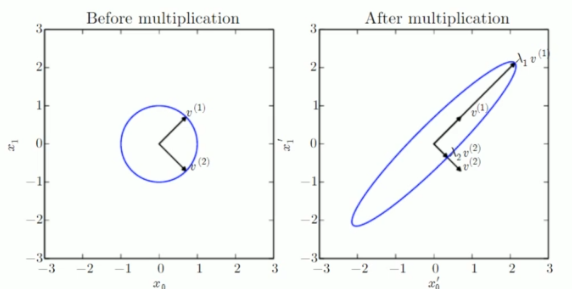
\includegraphics[width=0.8\textwidth]{gambar/gmb2.png}
    \caption{Perkalian antar dua buah vektor ortonormal eigen: $\mathbf{v^1}$ dan $\mathbf{v^2}$ dengan matriks $\mathbf{A}$ mengubah lingkaran satuan (\textit{unit circle}).}
    \label{fig:fig2}
\end{figure}

Dekomposisi eigen dimungkinkan jika matriks $\mathbf{A}$ mempunyai $n$ vektor - vektor eigen yang bersifat independen secara linier, sehingga kita dapat membentuk sebuah matriks $\mathbf{V}$ yang dengan sebuah vektor eigen per kolomnya dan sebuah vektor $\lambda$ yang memuat seluruh nilai - nilai eigen. Formulasi umum dari dekomposisi eigen untuk matriks $\mathbf{A}$ ditunjukkan pada persamaan \ref{eqn:eqn17} sebagai berikut:
\begin{equation}\label{eqn:eqn17}
    \mathbf{A} = \mathbf{V}\text{diag}(\lambda)\mathbf{V}^-1
\end{equation}

\subsection{Invers matriks}
Invers suatu matriks ($\mathbf{A}^{-1}$) digambarkan pada persamaan \ref{eqn:eqn18} berikut ini:

\begin{equation}\label{eqn:eqn18}
    \mathbf{A}.\mathbf{A}^{-1} = \mathbf{A}^{-1}.\mathbf{A} = \mathbf{I} 
\end{equation}
dimana $\mathbf{I}$ merupakan matriks identitas. Secara umum invers matriks ekuivalen dengan hubungan timbal-balik di dalam operasi perkalian di bilangan bulat.

\subsection{Sifat - sifat dekomposisi eigen}
Berikut adalah sifat - sifat dekomposisi eigen yang wajib kita pahami:


\begin{itemize}
    \item Dekomposisi eigen tidak dapat diterapkan pada seluruh matriks.
    \item Suatu matriks dikatakan matriks singular (tidak mempunyai invers) jika terdapat salah satu nilai eigen-nya yang bernilai nol.
    \item Suatu matriks yang mempunyai seluruh nilai eigen positif disebut sebagai definit positif.
    \item Suatu matriks yang mempunyai seluruh nilai eigen negatif disebut sebagai definit negatif.
\end{itemize}

\subsection{Motivasi penerapan dekomposisi eigen}
Dekomposisi eigen digunakan di dalam algoritma analisis komponen utama (\textit{Principle Component Analysis}: PCA). PCA merupakan prosedur statistik yang digunakan untuk mengubah suatu himpunan observasi dari variabel - variabel yang saling terkait menjadi suatu himpunan variabel yang secara linear tidak terkorelasi yang dinamakan komponen - komponen utama (\textit{principle components}). Secara umum dapat dikatakan bahwa PCA merupakan suatu metode yang digunakan untuk merangkum dan mengompresi data.

\section{Laboratorium 2: Norma dan dekomposisi eigen}
Pada catatan sebelumnya, kita telah membahas tentang konsep norma pada vektor dan matriks, normalisasi vektor, dan dekomposisi eigen. Pada bagian ini , kita akan menggunakan NumPy untuk mempermudah proses komputasinya dan memperkuat pemahaman kita akan konsep - konsep tersebut.

Seperti biasa, sebelum memulai kita harus memastikan bahwa kita menggunakan lingkungan komputasi yang sama:

\begin{pyin}
import sys
import numpy as np
from numpy import linalg

print('Python: {}'.format(sys.version))
print('NumPy: {}'.format(np.__version__))
\end{pyin}

\begin{pyout}
Python: 3.8.3 (default, May 19 2020, 18:47:26) 
[GCC 7.3.0]
NumPy: 1.18.1
\end{pyout}

\subsection{Norma vektor dan matriks}
Untuk menghitung norma vektor atau matriks, kita hanya cukup menggunakan satu baris perintah dengan fungsi \verb|linalg.norm()|:

\begin{pyin}
# mendefinisikan array
A = np.arange(9) - 3
A
\end{pyin}

\begin{pyout}
array([-3, -2, -1,  0,  1,  2,  3,  4,  5])
\end{pyout}

\begin{pyin}
# melakukan reshape membentuk matriks berukuran 3 x 3
B = A.reshape((3,3))
B
\end{pyin}

\begin{pyout}
array([[-3, -2, -1],
       [ 0,  1,  2],
       [ 3,  4,  5]])
\end{pyout}

\begin{pyin}
# Perhitungan Norma Euklidesan (L2)
print(np.linalg.norm(A))
print(np.linalg.norm(B))
\end{pyin}

\begin{pyout}
8.306623862918075
8.306623862918075
\end{pyout}

\begin{pyin}
# Perhitungan Norma Frobenius (L2 Norm untuk matriks)
print(np.linalg.norm(B, 'fro'))
\end{pyin}

\begin{pyout}
8.306623862918075
\end{pyout}

\begin{pyin}
# Perhitungan Norma L1
print(np.linalg.norm(A, 1))
print(np.linalg.norm(B, 1))
\end{pyin}

\begin{pyout}
21.0
8.0
\end{pyout}

\begin{pyin}
# Perhitungan norma maks (P = tak hingga)
print(np.linalg.norm(A, np.inf))
print(np.linalg.norm(B, np.inf))
\end{pyin}

\begin{pyout}
5.0
12.0
\end{pyout}

\subsection{Normalisasi vektor}
\begin{pyin}
# normalisasi untuk mendapatkan vektor satuan
norm = np.linalg.norm(A, 2)
sat_A = A / norm

print(sat_A)
\end{pyin}

\begin{pyout}
\%[-0.36115756 -0.24077171 -0.12038585  0.          0.12038585  0.24077171
  0.36115756  0.48154341  0.60192927]
\end{pyout}

\begin{pyin}
# norma dari vektor satuan adalah 1
np.linalg.norm(sat_A)
\end{pyin}

\begin{pyout}
1.0
\end{pyout}

\subsection{Dekomposisi eigen}
Kita dapat menghitung nilai dan vektor eigen dengan sangat mudah dengan menggunakan NumPy. Ingat bahwa vektor eigen dari matriks persegi $\mathbf{A}$ merupakan vektor bukan-nol $\mathbf{v}$, di mana perkalian dengan $\mathbf{A}$ hanya akan mengubah skalanya saja:

$$\mathbf{Av} = \lambda \mathbf{v}$$

Nilai skalar $\lambda$ dikenal sebagai nilai eigen.

\begin{pyin}
# mencari nilai dan vektor eigen untuk matriks persegi sederhana
A = np.diag(np.arange(1,4))
A
\end{pyin}

\begin{pyout}
array([[1, 0, 0],
       [0, 2, 0],
       [0, 0, 3]])
\end{pyout}

\begin{pyin}
nilai_eigen, vektor_eigen = np.linalg.eig(A)
print("Nilai - nilai eigen: {}".format(nilai_eigen))
print("Vektor - vektor eigen: {}".format(vektor_eigen))
\end{pyin}

\begin{pyout}
Nilai - nilai eigen: [1. 2. 3.]
Vektor - vektor eigen: [[1. 0. 0.]
 [0. 1. 0.]
 [0. 0. 1.]]
\end{pyout}

\begin{pyin}
# nilai eigen w[i] berkorespondensi pada vektor eigen v[:, i]
print('Nilai eigen: {}'.format(nilai_eigen[1]))
print('Vektor eigen: {}'.format(vektor_eigen[:,1]))
\end{pyin}

\begin{pyout}
Nilai eigen: 2.0
Vektor eigen: [0. 1. 0.]
\end{pyout}

Kita dapat dengan mudah melakukan pengecekan kembali pada nilai dan vektor eigen ini dengan melakukan perhitungan sebagai berikut:
 $$\textbf{A} = \textbf{V}diag(\lambda)\textbf{V}^{-1}$$
\begin{pyin}
# verifikasi - dekomposisi eigen untuk menghasilkan nilai A

matriks = np.matmul(np.diag(nilai_eigen), np.linalg.inv(vektor_eigen))
A = np.matmul(vektor_eigen, matriks).astype(np.int)
print(A)
\end{pyin}

\begin{pyout}
\%[[1 0 0]
 [0 2 0]
 [0 0 3]]
\end{pyout}

Nilai dan vektor eigen umumnya sulit untuk dipahami secara konseptual, untuk itu pada contoh berikut ini, kita mencoba memvisualisasikan perkalian antara vektor - vektor eigen dengan matriks $A$ dengan menggunakan pustaka matplotlib.

\begin{pyin}
# mengimpor pustaka - pustaka yang diperlukan untuk visualisasi data
import matplotlib.pyplot as plt
from mpl_toolkits.mplot3d import Axes3D
import matplotlib.cm as cm
\%matplotlib inline
\end{pyin}

\begin{pyin}
# plot vektor - vektor eigen
titik_awal = [0,0,0]

fig = plt.figure(figsize=(18,10))
ax1 = fig.add_subplot(121, projection='3d')

ax1.quiver(titik_awal, titik_awal, titik_awal, vektor_eigen[0, :], vektor_eigen[1, :], vektor_eigen[2, :], color = 'k')
ax1.set_xlim([-3, 3])
ax1.set_ylim([-3, 3])
ax1.set_zlim([-3, 3])
ax1.set_xlabel('sumbu-$x$')
ax1.set_ylabel('sumbu-$y$')
ax1.set_zlabel('sumbu-$z$')
ax1.view_init(15, 30)
ax1.set_title("Sebelum Perkalian")

# perkalian matriks awal dengan vektor - vektor eigen
eig_baru = np.matmul(A, vektor_eigen)
ax2 = plt.subplot(122, projection='3d')

# plot vektor - vektor baru
ax2.quiver(titik_awal, titik_awal, titik_awal, eig_baru[0, :], eig_baru[1, :], eig_baru[2, :], color = 'k')

# plot nilai - nilai eigen untuk setiap vektor 
ax2.plot((nilai_eigen[0]*vektor_eigen[0]), (nilai_eigen[1]*vektor_eigen[1]), (nilai_eigen[2]*vektor_eigen[2]), 'rX')
ax2.set_title("Sesudah Perkalian")
ax2.set_xlim([-3, 3])
ax2.set_ylim([-3, 3])
ax2.set_zlim([-3, 3])
ax2.set_xlabel('sumbu-$x$')
ax2.set_ylabel('sumbu-$y$')
ax2.set_zlabel('sumbu-$z$')
ax2.view_init(15, 30)

# tampilkan plot!
plt.show()
\end{pyin}

\begin{figure}[H]
    \centering
    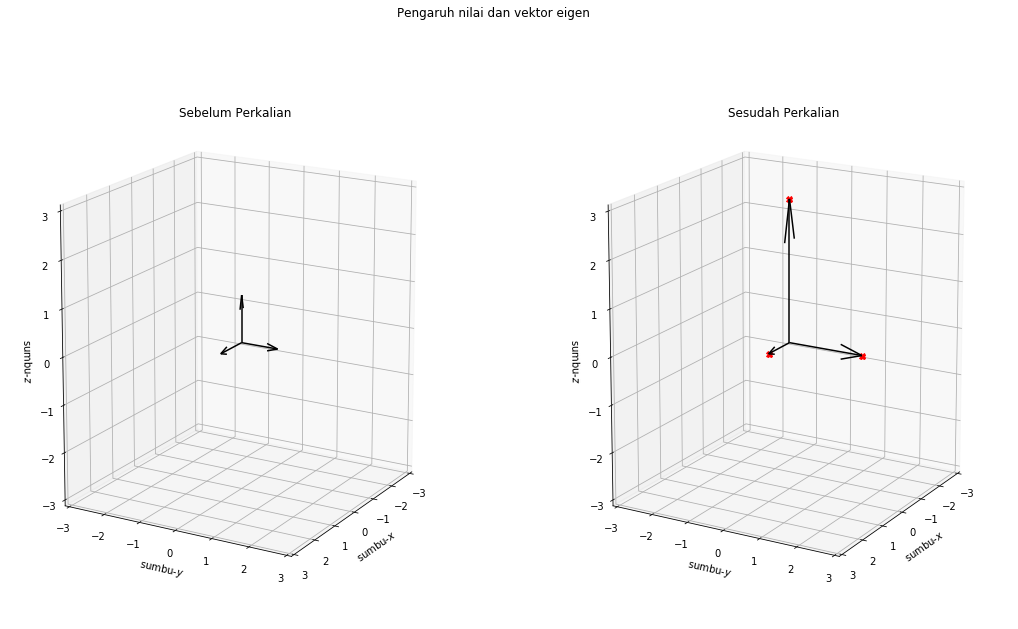
\includegraphics[width=1\textwidth]{gambar/gmb3.png}
    \caption{Pengaruh nilai dan vektor eigen.}
    \label{fig:fig3}
\end{figure}